\documentclass[tikz,convert={outfile=\jobname.svg}]{standalone}
%\usetikzlibrary{...}% tikz package already loaded by 'tikz' option
\usetikzlibrary{mindmap,trees}
\begin{document}
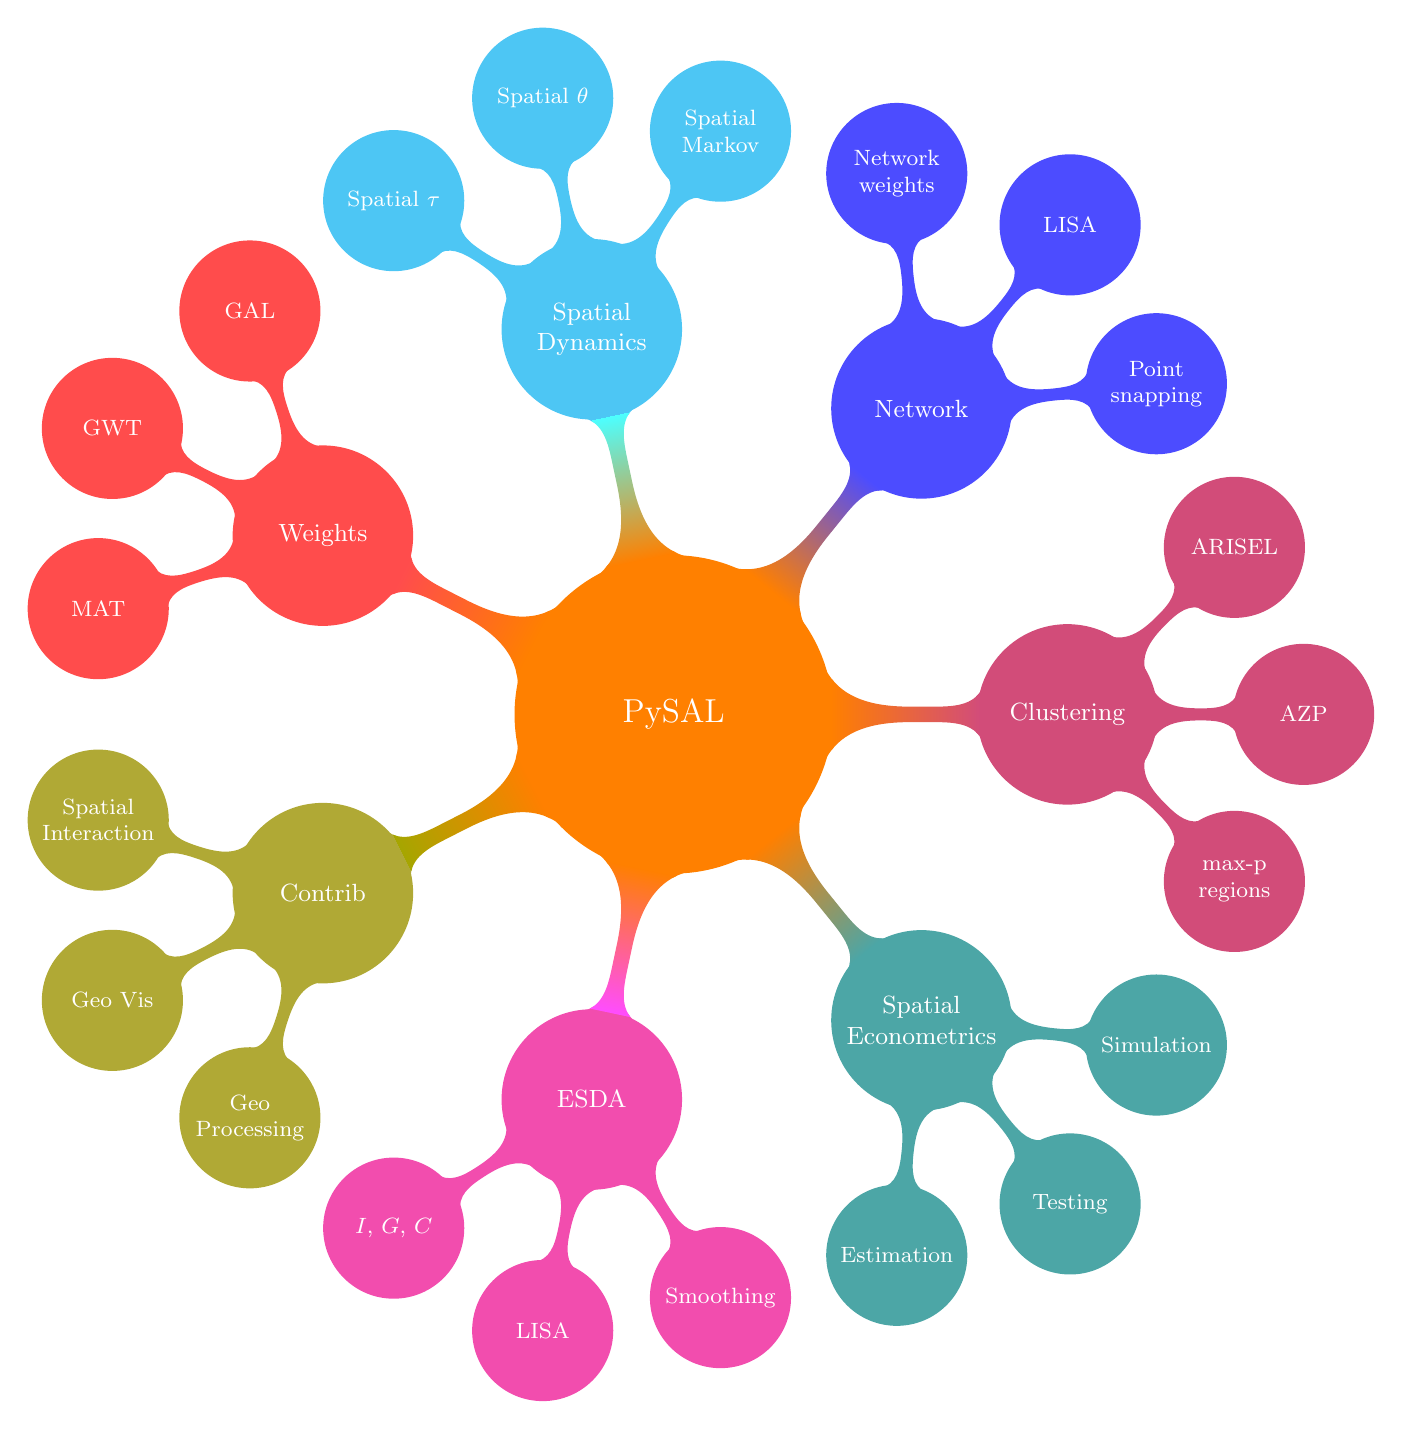
\begin{tikzpicture}[mindmap,grow cyclic, every node/.style=concept, concept color=orange,text=white,
  level 1/.append style={level distance=5cm, sibling angle=51},
  level 2/.append style={level distance=3cm,sibling angle=45},]
    \node{PySAL}
	child [concept color=olive!70]{ node {Contrib}
		child { node {Spatial Interaction}}
		child { node {Geo Vis}}
		child { node {Geo Processing}}
	}
    	child [concept color=magenta!70] { node {ESDA}
		child { node {$I$, $G$, $C$}}
		child { node {LISA}}
		child { node {Smoothing}}
	}
	child [concept color=teal!70] { node {Spatial Econometrics}
		child { node {Estimation}}
		child { node {Testing}}
		child { node {Simulation}}
	}
	child [concept color=purple!70]{ node {Clustering}
		child { node {max-p regions}}
		child { node {AZP}}
		child { node {ARISEL}}
	}
	child [concept color=blue!70]{ node {Network}
		child { node {Point snapping}}
		child { node {LISA}}
		child { node {Network weights}}
	}
	child [concept color=cyan!70]{ node {Spatial Dynamics}
		child { node {Spatial Markov}}
		child { node {Spatial $\theta$}}
		child { node {Spatial $\tau$}}
	}
	child [concept color=red!70]{ node {Weights}
		child { node {GAL}}
		child { node {GWT}}
		child { node {MAT}}
	}
    	;
\end{tikzpicture}
\end{document}
